\documentclass[report]{subfiles}

\begin{document}
\label{sec:result}
The following section contains the results of the KNN and Random Forest algorithms.

\subsection{KNN}
\label{sec:resultKNN}
The result of the easy problem with KNN can be seen at figure~\ref{fig:knnEasyProblem}. The setting with 'sigma = 1' in smoothing and 0.99 principle components gives a success of approx 86\% with k as 1.\\
One thing to note is that there are not a big difference with the k-values, they are however slowly dropping in success the higher a k-value.

\begin{figure}[H]
	\centering
	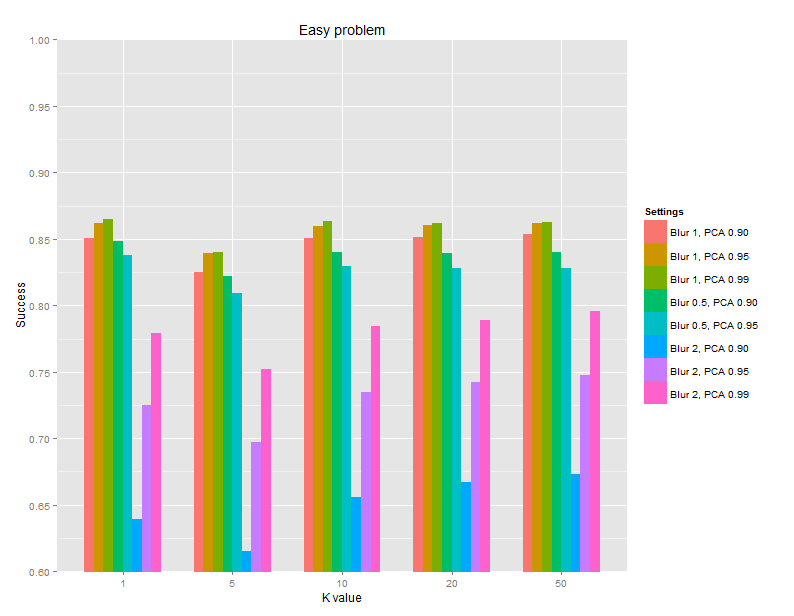
\includegraphics[width=1\textwidth]{images/knnEasyProblem}
	\caption{Figure of the result after running KNN on the easy problem}
	\label{fig:knnEasyProblem}
\end{figure}

The best settings from the easy problem was then used with the hard problem, and the results can be seen at figure~\ref{fig:knnHardProblem}, where the best hand writing is at approx 84\% success and the worst is at approx 42\%. Running with different k-values and PCA percentages did not change much, it was still the same two people low in the success and the same two to three with the highest success.

\begin{figure}[H]
	\centering
	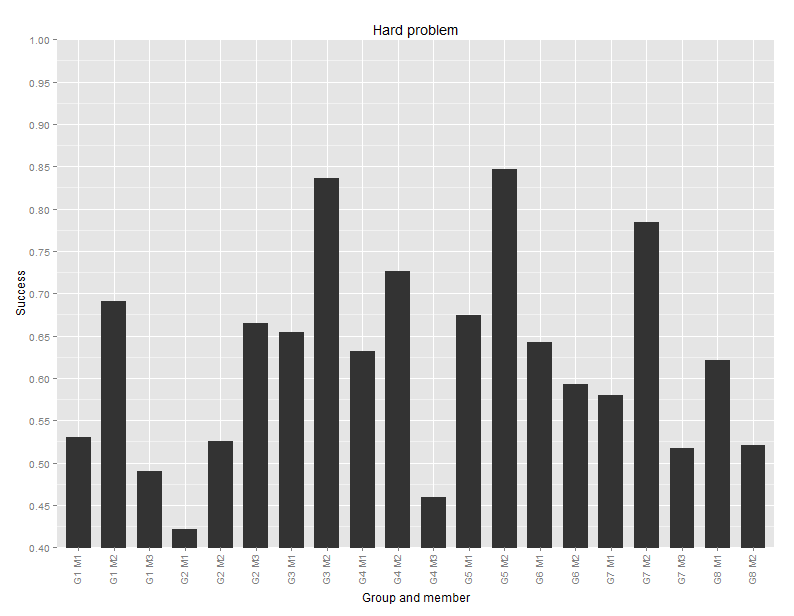
\includegraphics[width=1\textwidth]{images/knnHardProblem}
	\caption{Figure of the result after running KNN on the hard problem}
	\label{fig:knnHardProblem}
\end{figure}

\subsection{Random Forest}
\label{sec:resultRandomForest}
The results for Random Forest is in the below sections \ref{sec:resultRandomForest:EasyProblem} and \ref{sec:resultRandomForest:HardProblem}.

\subsubsection{Easy Problem}
\label{sec:resultRandomForest:EasyProblem}
The result of the easy problem with Random Forest is illustrated in figure~\ref{fig:rfEasyProblem}. 

The best result with using PC's from the PCA is with 95 \% coverage of variance and sigma value of 1, which yielded a accuracy of 84.04 \%.

There seem to be a local maximum for 95 \% coverage which drops, when going to either 90 and 99 \%.

For Kmeans the most approbiate amount of clusters seem to be around ?? 

\begin{figure}[H]
  \centering
  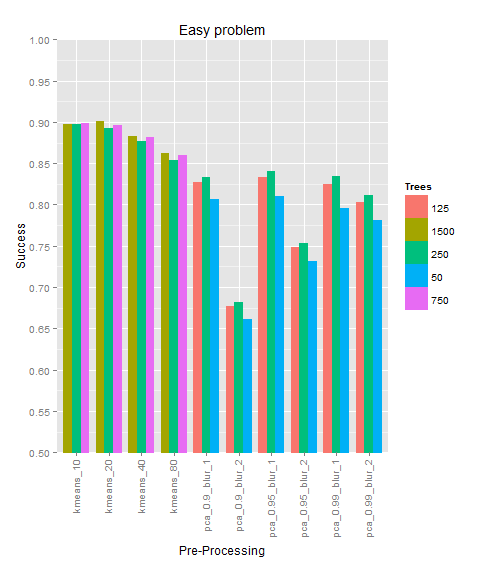
\includegraphics[width=1\textwidth]{images/rf_easy}
  \caption{Figure showing performance using the Random Forest algorithm, with different pre prosessing and parameters}
  \label{fig:rfEasyProblem}
\end{figure}

\subsubsection{Hard Problem}
\label{sec:resultRandomForest:HardProblem}

The setting stated in section~\ref{sec:implRF:hardProblem} yielded the results shown in figure~\ref{fig:rfHardProblem}. 

A funny occourence shows that for the two approaches, different people both the worst hand writing and the best.

\begin{figure}[H]
  \centering
  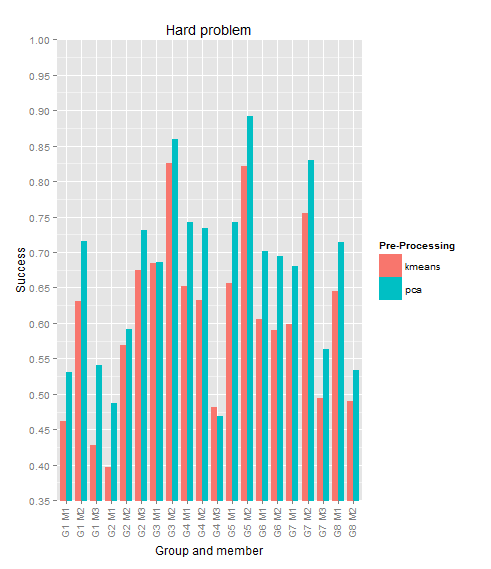
\includegraphics[width=1\textwidth]{images/rf_hard}
  \caption{Figure showing performance using the Random Forest algorithm, having each person as test}
  \label{fig:rfHardProblem}
\end{figure}

With KMeans pre-processing, the best/worst was:
\begin{description}
\item[Best] Group 3, Member 2
\item[Worst] Group 2, Member 1
\end{description}

With PCA pre-processing, the best/worst was:
\begin{description}
\item[Best] Group 5, Member 2
\item[Worst] Group 4, Member 3
\end{description}


This indicates that different results could be proven using different pre-processing, which favors some peoples hand-writing over others. 

In all PCA caused the best results overall, where only Group 4, Member 3 achieved a higher performance in KMeans in contrast to PCA.

\subsection{Who has the worst hand writing?}
One of the goals for the course was to figure out who has the worst hand writing, it was however not possible say that one specific person has the worst hand writing, instead it can be seen from the results that it is the same few people who evaluate at the bottom.
\begin{itemize}
	\item KNN: First place is member 1 from group 2 at 42\%, with the runner up as member 3 from group 4 at 46\%.
	\item Random Forest with PCA: First place is member 3 from group 4 at 46\% and the runner up is member 1 from group 2 at 47\%.
	\item Random Forest with K-Means: First place is member 1 from group 2 at 39\% and the runner up is member member 3 from group 1 at 43\%.
\end{itemize}
The conclusion must therefore be that \textbf{member 1 from group 2} and \textbf{member 3 from group 4} has the worst hand writings!

\end{document}